\chapter{علم البلورات وحيود الأشعة السينية}\label{ch:b3:x-ray-diffraction}

في سنة 1912 ترك شعاع من الأشعة السينية أُرسل عبر بلورة من كبريتات النحاس على
لوح فوتوغرافي نمطًا من البقع الحادة: فالبلورات تحيد الأشعة السينية كما
يحيد المحزوز الضوء، لأن المسافات بين ذراتها
تضاهي طول موجة الأشعة السينية. وبعد سنة قرأ ويليام لورنس براغ، وكان يومئذ
طالبًا، من مثل هذه الأنماط بنية الملح الصخري --- وبيّن أن
الصلب لا يحتوي على أي جزيء \ce{NaCl}، بل على شبكة فقط يحيط فيها بكل أيون
ستة جيران من النوع الآخر. وكل بنية بلورية ورد ذكرها في
مجلد السنة الأولى وفي هذا الكتاب اكتُشفت بهذه الطريقة. ويقدّم هذا الفصل
هندسة الشبكات وتناظرها، وشرط الحيود، 
والشدات التي تكشف محتوى الخلية، وطريقتي المسحوق
والبلورة المفردة المستعملتين في كل مختبر.

\begin{recall}
وصف مجلد السنة الأولى البلورات بشبكة من العقد ونقش وخلية
أولية بوسائط شبكتها؛ وعدّ تعددية الخلية؛ وبنى
البنى المكعبة الممركزة الأوجه والممركزة الجسم والسداسية المتراصة
وأنماط الملح الصخري وكلوريد السيزيوم وبلندة الزنك والفلوريت؛ 
وحسب الكثافة من الخلية. وعرّف \cref{ch:b3:point-groups}
\omterm{def:b3:point-groups:operation}{عمليات التناظر} والزمر النقطية.
\end{recall}

\begin{omfigure}
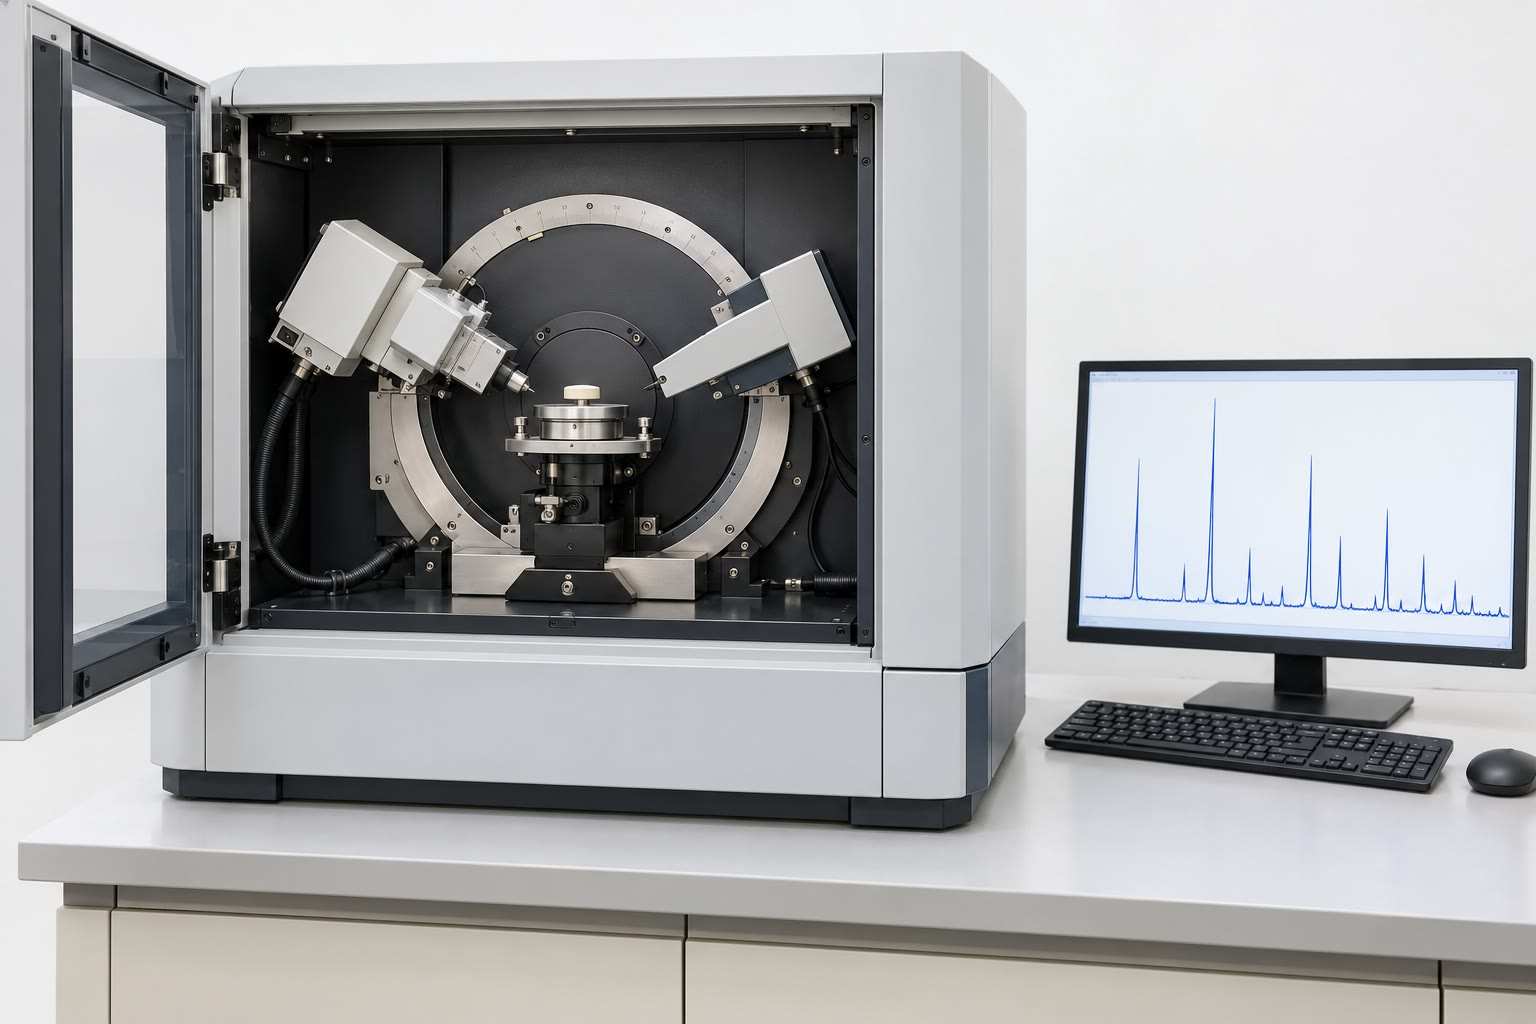
\includegraphics[width=0.6\linewidth]{images/book4/ai/b3-09-diffractometer.jpg}

{\small جهاز حيود مسحوق مكتبي: أنبوب الأشعة السينية والكاشف
يدوران على دائرة حول العيّنة المسطحة.}
\end{omfigure}

\section{الأنظمة البلورية وشبكات برافيه}

لا يمكن أن تكون للشبكة إلا عمليات تناظر تنقل الشبكة إلى نفسها.
وهذا يقيّدها تقييدًا شديدًا.

\begin{theorem}[القيد البلوري]\label{thm:b3:x-ray-diffraction:restriction}
محاور الدوران الوحيدة المتوافقة مع شبكة هي ذات الرتب 1 و2 و3 و4 و6.
\end{theorem}

\begin{proof}
في أساس من متجهات الشبكة، ينقل دوران التناظر متجهات الشبكة إلى
متجهات الشبكة، فعناصر مصفوفته أعداد صحيحة وأثرها عدد صحيح. 
والأثر لا يتعلق بالأساس؛ وفي أساس متعامد منظَّم يكون فيه $z$ على امتداد
المحور يساوي $1 + 2\cos\theta$. ومنه $2\cos\theta$ عدد صحيح بين $-2$ و2:
$\cos\theta \in \{-1, -\frac12, 0, \frac12, 1\}$، $\theta = 180^\circ, 120^\circ, 90^\circ,
60^\circ, 0^\circ$: أي الرتب 2 و3 و4 و6 و1. فالمحور الخماسي مستحيل.
\end{proof}

\begin{definition}[النظام البلوري، شبكة برافيه، تمركز الشبكة]\label{def:b3:x-ray-diffraction:crystal-system}
تُجمَّع الشبكات بحسب تناظرها في سبعة \emph{أنظمة
بلورية}\index{نظام بلوري} (ثلاثي الميل، أحادي الميل، معيني قائم، رباعي،
ثلاثي، سداسي، مكعب). يمكن أن تحمل الخلية عقدًا شبكية في رؤوسها فقط
(أولية، P) أو أيضًا في مركزها (ممركزة الجسم، I)، أو في مراكز كل
الأوجه (ممركزة الأوجه، F) أو في مركزي زوج واحد من الأوجه (ممركزة القاعدة، C)، أو على امتداد
قطر أكبر (معينية الأوجه، R): وهذا هو \emph{تمركز
الشبكة}\index{تمركز الشبكة}. والتركيبات المختلفة الأربع عشرة لنظام 
وتمركز هي \emph{شبكات برافيه}\index{شبكة برافيه}.
\end{definition}

\begin{center}\small
\begin{tabular}{lll}
\hline
النظام & قيود الخلية & التمركزات \\ \hline
ثلاثي الميل & لا قيود & P \\
أحادي الميل & $\alpha = \gamma = 90^\circ$ & P، C \\
معيني قائم & $\alpha = \beta = \gamma = 90^\circ$ & P، C، I، F \\
رباعي & $a = b$، كل الزوايا $90^\circ$ & P، I \\
ثلاثي & $a = b = c$، $\alpha = \beta = \gamma \ne 90^\circ$ (محاور معينية الأوجه) & R \\
سداسي & $a = b$، $\alpha = \beta = 90^\circ$، $\gamma = 120^\circ$ & P \\
مكعب & $a = b = c$، كل الزوايا $90^\circ$ & P، I، F \\ \hline
\end{tabular}
\end{center}

\begin{omfigure}
\tdplotsetmaincoords{60}{100}
\begin{tikzpicture}[tdplot_main_coords, scale=1.25, font=\small]
  \foreach \s/\lab in {0/{\foreignlanguage{arabic}{مكعب P}}, 3.0/{\foreignlanguage{arabic}{مكعب I}}, 6.0/{\foreignlanguage{arabic}{مكعب F}}}{
    \begin{scope}[xshift=\s cm]
      \pic[transform shape] {omcubeo={1.6}};
      \foreach \x in {0,1.6}{\foreach \y in {0,1.6}{\foreach \z in {0,1.6}{\node[cellA=2.6mm] at (\x,\y,\z) {};}}}
      \node[anchor=north] at (0.8,0.8,-0.62) {\lab};
    \end{scope}}
  \begin{scope}[xshift=3.0cm]
    \node[cellB=2.6mm] at (0.8,0.8,0.8) {};
  \end{scope}
  \begin{scope}[xshift=6.0cm]
    \foreach \p in {(0.8,0.8,0),(0.8,0.8,1.6),(0.8,0,0.8),(0.8,1.6,0.8),(0,0.8,0.8),(1.6,0.8,0.8)}{\node[cellB=2.6mm] at \p {};}
  \end{scope}
\end{tikzpicture}

{\small \omterm{def:b3:x-ray-diffraction:crystal-system}{شبكات برافيه} المكعبة الثلاث: الأولية (عقد في الرؤوس)،
والممركزة الجسم (يضاف إليها المركز، بالأحمر) والممركزة الأوجه (يضاف إليها مراكز
الأوجه الستة، بالأحمر). وتحمل خلاياها 1 و2 و4 عقد.}
\end{omfigure}

\section{المستويات الشبكية والشبكة المقلوبة}

\begin{definition}[المستوي الشبكي، قرائن ميلر، المسافة بين المستويات]\label{def:b3:x-ray-diffraction:miller}
\emph{المستوي الشبكي}\index{مستوي شبكي} مستوٍ يمر بثلاث عقد على الأقل
غير واقعة على استقامة واحدة؛ وهو ينتمي إلى عائلة من المستويات المتوازية المتساوية التباعد
التي تحتوي كل العقد. وإذا قطع أقرب مستويات العائلة إلى المبدأ
المحاور عند $a/h$ و$b/k$ و$c/l$، فالأعداد الصحيحة $(hkl)$، دون قاسم مشترك،
هي \emph{قرائن ميلر}\index{قرائن ميلر} له (القرينة 0 لمستوٍ
موازٍ لمحور). والمسافة بين مستويين متجاورين هي
\emph{المسافة بين المستويات}\index{المسافة بين المستويات} $d_{hkl}$.
\end{definition}

\begin{proposition}[المسافات في الخلايا المتعامدة المحاور]\label{prop:b3:x-ray-diffraction:spacing}
من أجل خلية معينية قائمة، $\dfrac{1}{d_{hkl}^2} = \dfrac{h^2}{a^2} + \dfrac{k^2}{b^2} +
\dfrac{l^2}{c^2}$؛ ومن أجل خلية مكعبة، $d_{hkl} = a/\sqrt{h^2 + k^2 + l^2}$.
\end{proposition}

\begin{proof}
للمستوي $hx/a + ky/b + lz/c = 1$ متجهة ناظمية $\mathbf n = (h/a, k/b, l/c)$
ويقع على مسافة $1/|\mathbf n|$ من المبدأ؛ والمستوي الموازي المار
بالمبدأ ينتمي إلى العائلة، ومنه $d = 1/|\mathbf n|$.
\end{proof}

\begin{definition}[الشبكة المقلوبة]\label{def:b3:x-ray-diffraction:reciprocal}
من أجل شبكة متجهات أساسها $\mathbf a$ و$\mathbf b$ و$\mathbf c$ وحجم خليتها $V$،
تكون متجهات أساس \emph{الشبكة المقلوبة}\index{شبكة مقلوبة}
$\mathbf a^* = (\mathbf b\times\mathbf c)/V$، $\mathbf b^* = (\mathbf c\times\mathbf a)/V$،
$\mathbf c^* = (\mathbf a\times\mathbf b)/V$، بحيث $\mathbf a\cdot\mathbf a^* = 1$ 
و$\mathbf a\cdot\mathbf b^* = 0$. وعقدتها $\mathbf G_{hkl} = h\mathbf a^* + k\mathbf b^* + l\mathbf c^*$
عمودية على المستويات $(hkl)$، و$|\mathbf G_{hkl}| = 1/d_{hkl}$.
\end{definition}

\section{الحيود}

\begin{theorem}[قانون براغ]\label{thm:b3:x-ray-diffraction:bragg}
لا تنعكس الأشعة السينية ذات طول الموجة $\lambda$ على عائلة من المستويات المتباعدة بمسافة $d$
إلا عند زوايا الانزلاق $\theta$ التي تحقق
\[
2d\sin\theta = n\lambda, \qquad n = 1, 2, \dots,
\]
وهو \emph{قانون براغ}\index{قانون براغ}. وتُدمج الرتبة $n$ بكتابة
الانعكاس $(nh\,nk\,nl)$ بمسافة $d/n$.
\end{theorem}

\begin{proof}
الأشعة التي ينثرها مستويان متجاوران، بزاويتي ورود 
وانعكاس متساويتين $\theta$، يختلف مسيراها بمقدار $2d\sin\theta$ (القطعتان على جانبي
الناظم المار بالمستوي الأدنى). وهي تتقوى حين يكون هذا الفرق
عددًا صحيحًا من أطوال الموجة؛ ومع ملايين المستويات، تعطي أي زاوية أخرى
أشعة يُلغي بعضها بعضًا مثنى مثنى.
\end{proof}

\begin{omfigure}
\begin{tikzpicture}[font=\small, >=Stealth]
  \foreach \y in {0,-1.1}{\draw[thick] (-0.4,\y) -- (7.4,\y);}
  \foreach \x in {0,1.4,...,7.0}{\fill (\x,0) circle (1.5pt) (\x,-1.1) circle (1.5pt);}
  \draw[->, omDef, thick] (0.2,1.75) -- (2.8,0);
  \draw[->, omDef, thick] (2.8,0) -- (5.4,1.75);
  \draw[->, omDef, thick] (-1.43,1.75) -- (2.8,-1.1);
  \draw[->, omDef, thick] (2.8,-1.1) -- (7.03,1.75);
  \draw[densely dashed] (2.8,0) -- (2.8,-1.1);
  \draw[omThm, thick] (2.8,0) -- (2.18,-0.68) (2.8,0) -- (3.42,-0.68);
  \draw[omThm, very thick] (2.18,-0.68) -- (2.8,-1.1) -- (3.42,-0.68);
  \draw (1.8,0) arc[start angle=180, end angle=213.9, radius=1.0];
  \node[anchor=east] at (1.85,-0.2) {$\theta$};
  \draw[<->] (7.7,0) -- (7.7,-1.1) node[midway, right] {$d$};
  \node[omThm, anchor=north] at (2.8,-1.2) {\foreignlanguage{arabic}{فرق المسير $2d\sin\theta$}};
\end{tikzpicture}

{\small إنشاء براغ. تقطع الأشعة المنعكسة على مستويين متجاورين
مسافة أطول بمقدار القطعتين الحمراوين، $d\sin\theta$ لكل منهما؛ وتتقوى الموجات حين يكون
$2d\sin\theta$ عددًا صحيحًا من أطوال الموجة.}
\end{omfigure}

\begin{proposition}[شرط لاوه]\label{prop:b3:x-ray-diffraction:laue}
مع متجهتي الموجة الواردة والمنتثرة $\mathbf k$ و$\mathbf k'$ اللتين طولهما
$1/\lambda$، يحدث الحيود حين $\mathbf k' - \mathbf k = \mathbf G_{hkl}$، وهي متجهة من
\omterm{def:b3:x-ray-diffraction:reciprocal}{الشبكة المقلوبة}؛ وهذا مكافئ \omterm{thm:b3:x-ray-diffraction:bragg}{لقانون براغ}.
\end{proposition}

\begin{proof}
الموجات التي تنثرها عقدتان يفصل بينهما متجهة شبكية $\mathbf R$ تختلف في الطور
بمقدار $2\pi(\mathbf k' - \mathbf k)\cdot\mathbf R$؛ وتتقوى كلها إذا كان هذا مضاعفًا للعدد $2\pi$
من أجل كل $\mathbf R$، أي إذا كانت $\mathbf k' - \mathbf k$ في \omterm{def:b3:x-ray-diffraction:reciprocal}{الشبكة المقلوبة} (بحسب
التعريف $\mathbf a\cdot\mathbf a^* = 1$، $\mathbf a\cdot\mathbf b^* = 0$\dots). ومن أجل انتثار مرن،
$|\mathbf k| = |\mathbf k'|$ و$|\mathbf k' - \mathbf k| = 2\sin\theta/\lambda$، حيث $2\theta$ الزاوية
بينهما؛ ومع $|\mathbf G| = 1/d$ يصير هذا $2d\sin\theta = \lambda$، و$\mathbf G$ ناظمية على
المستويات العاكسة.
\end{proof}

\begin{definition}[كرة إيفالد]\label{def:b3:x-ray-diffraction:ewald}
\emph{كرة إيفالد}\index{كرة إيفالد} نصف قطرها $1/\lambda$ وتمر
بمبدأ \omterm{def:b3:x-ray-diffraction:reciprocal}{الشبكة المقلوبة}، ومركزها عند $-\mathbf k$ من المبدأ؛ ويحدث
انعكاس كلما وقعت عليها عقدة من \omterm{def:b3:x-ray-diffraction:reciprocal}{الشبكة المقلوبة}.
\end{definition}

\begin{omfigure}
\begin{tikzpicture}[font=\small, >=Stealth, scale=0.9]
  \foreach \i in {-2,...,4}{\foreach \j in {-2,...,2}{\fill[black!60] (\i*1.0,\j*0.75) circle (1.3pt);}}
  \node[anchor=north east] at (0,0) {$O$};
  \draw[omDef] (-1.625,0.0) circle (1.625);
  \draw[->, omDef, thick] (-1.625,0) -- (0,0) node[midway, below] {$\mathbf k$};
  \draw[->, omThm, thick] (-1.625,0) -- (-1.0,1.5);
  \node[omThm, anchor=east] at (-1.4,0.85) {$\mathbf k'$};
  \draw[->, black, very thick] (0,0) -- (-1.0,1.5) node[pos=0.3, left] {$\mathbf G$};
  \node[anchor=north] at (-1.625,-1.75) {\foreignlanguage{arabic}{كرة إيفالد، نصف قطرها $1/\lambda$}};
  \draw[<->] (4.6,0) -- (4.6,0.75) node[midway, right] {$b^*$};
  \draw[<->] (3,-1.85) -- (4,-1.85) node[midway, below] {$a^*$};
\end{tikzpicture}

{\small إنشاء إيفالد في بعدين (تمر الدائرة بالمبدأ
$O$ \omterm{def:b3:x-ray-diffraction:reciprocal}{للشبكة المقلوبة}). العقدة $\mathbf G$ الواقعة على الدائرة تعطي
حزمة محيدة $\mathbf k' = \mathbf k + \mathbf G$. وهنا تمر الدائرة، التي اختير نصف قطرها
لأجل الرسم، بالعقدة $(-1, 2)$.}
\end{omfigure}

\section{الشدات والتناظر}

يعطي \omterm{thm:b3:x-ray-diffraction:bragg}{قانون براغ} اتجاهات الحزم المحيدة، وهي لا تتعلق إلا
بالشبكة؛ أما شداتها فتتعلق بما في الخلية.

\begin{definition}[عامل الانتثار الذري، عامل البنية]\label{def:b3:x-ray-diffraction:structure-factor}
\emph{عامل الانتثار الذري}\index{عامل الانتثار الذري} $f_j$ لذرة
هو السعة التي تنثرها، مقيسةً بسعة إلكترون واحد؛ وهو يساوي
عدد إلكتروناتها في الاتجاه الأمامي ويتناقص عند الزوايا
الأكبر. و\emph{عامل البنية}\index{عامل البنية} للانعكاس $hkl$ هو
\[
F_{hkl} = \sum_jf_j\,\eu^{2\pi\iu(hx_j + ky_j + lz_j)},
\]
مجموعًا على ذرات الخلية ذات الإحداثيات الكسرية $(x_j, y_j, z_j)$.
\end{definition}

\begin{proposition}[الشدة]\label{prop:b3:x-ray-diffraction:intensity}
شدة الانعكاس متناسبة مع $|F_{hkl}|^2$.
\end{proposition}

\begin{proof}[برهان جزئي]
تقع الذرة $j$ عند $\mathbf r_j = x_j\mathbf a + y_j\mathbf b + z_j\mathbf c$؛ ومن أجل انعكاس،
$(\mathbf k' - \mathbf k)\cdot\mathbf r_j = hx_j + ky_j + lz_j$، فلموجتها الطور
$2\pi(hx_j + ky_j + lz_j)$ بالنسبة إلى ذرة في المبدأ، والسعة $f_j$:
فتنثر الخلية المجموع $F_{hkl}$، وكل خلية الشيء نفسه. والشدة هي
مربع طويلة السعة. أما إمكان إهمال الانتثار المتعدد
(التقريب الحركي) فنقبله دون برهان.
\end{proof}

\begin{definition}[الغياب المنهجي]\label{def:b3:x-ray-diffraction:absence}
\emph{الغياب المنهجي}\index{غياب منهجي} انعكاس ينعدم عامل
بنيته في كل بلورة ذات تمركز شبكي أو
تناظر معين، أيًا كانت ذراتها.
\end{definition}

\begin{proposition}[غيابات الشبكات الممركزة]\label{prop:b3:x-ray-diffraction:absences}
في الشبكة الممركزة الجسم، تغيب الانعكاسات ذات $h + k + l$ فردي؛ وفي
الشبكة الممركزة الأوجه، تغيب الانعكاسات ذات $h$ و$k$ و$l$ المختلطة الزوجية.
\end{proposition}

\begin{proof}
التمركز I: لكل ذرة عند $(x,y,z)$ نسخة عند $(x + \frac12, y + \frac12, z + \frac12)$،
يختلف عامل طورها بالعامل $\eu^{\iu\pi(h+k+l)} = (-1)^{h+k+l}$: $F = (1 +
(-1)^{h+k+l})F'$. التمركز F: النسخ عند مراكز ثلاثة أوجه تعطي العامل $1 +
(-1)^{h+k} + (-1)^{h+l} + (-1)^{k+l}$، الذي يساوي 4 إذا كانت $h$ و$k$ و$l$ كلها زوجية أو كلها فردية
ويساوي 0 فيما عدا ذلك.
\end{proof}

\begin{example}[الملح الصخري والسيلفيت]\label{ex:b3:x-ray-diffraction:nacl-kcl}
% ledger: lat:NaCl, lat:KCl
في بنية الملح الصخري، الكاتيونات عند $(0,0,0)$ والأنيونات عند $(\frac12,0,0)$، ولكل منها
انسحابات F: $F_{hkl} = 4[f_+ + f_-(-1)^{h+k+l}]$ من أجل القرائن غير المختلطة.
ومن أجل \ce{NaCl}، $f(\ce{Na+}) \approx 10$ و$f(\ce{Cl-}) \approx 18$: فالانعكاسات الفردية كلها
(111) و(311) ضعيفة لكنها حاضرة. ومن أجل \ce{KCl}، لكل من \ce{K+} و\ce{Cl-} ثمانية عشر
إلكترونًا: فتكاد الانعكاسات الفردية كلها تختفي، ويبدو النمط كأنه
نمط شبكة مكعبة أولية حرفها نصف حرف الخلية (الشكل أدناه).
\end{example}

\begin{omfigure}
\begin{tikzpicture}
\begin{axis}[name=salts, width=0.95\linewidth, height=5.2cm, xmin=20, xmax=90,
  ymin=0, ymax=2.55, ytick=\empty, axis x line=bottom, axis y line=none,
  xlabel={\foreignlanguage{arabic}{\babelsublr{$2\theta$} بالدرجات \babelsublr{(Cu K$\alpha_1$)}}}, tick label style={font=\small},
  label style={font=\small}]
\addplot[omDef, thin] table[x=tt, y expr=\thisrow{NaCl}+1.35] {figdata/out/bachelor-3-xrd-powder-salts.dat};
\addplot[omThm, thin] table[x=tt, y=KCl] {figdata/out/bachelor-3-xrd-powder-salts.dat};
\node[font=\small, omDef, anchor=west] at (axis cs:79,1.9) {\ce{NaCl}};
\node[font=\small, omThm, anchor=west] at (axis cs:77,0.55) {\ce{KCl}};
\node[font=\scriptsize, anchor=south] at (axis cs:27.36,1.52) {111};
\node[font=\scriptsize, anchor=west] at (axis cs:32.1,2.25) {200};
\node[font=\scriptsize, anchor=west] at (axis cs:28.8,0.9) {200};
\node[font=\scriptsize, anchor=west] at (axis cs:41.0,0.85) {220};
\end{axis}
\end{tikzpicture}

\begin{tikzpicture}
\begin{axis}[name=met, width=0.62\linewidth, height=4.4cm, xmin=35, xmax=100,
  ymin=0, ymax=2.35, ytick=\empty, axis x line=bottom, axis y line=none,
  xlabel={\foreignlanguage{arabic}{\babelsublr{$2\theta$} بالدرجات}}, tick label style={font=\small}, label style={font=\small}]
\addplot[omDef, thin] table[x=tt, y expr=\thisrow{Cu}+1.2] {figdata/out/bachelor-3-xrd-powder-metals.dat};
\addplot[omThm, thin] table[x=tt, y=W] {figdata/out/bachelor-3-xrd-powder-metals.dat};
\node[font=\small, omDef, anchor=west] at (axis cs:55,1.5) {Cu (F)};
\node[font=\small, omThm, anchor=west] at (axis cs:44,0.4) {W (I)};
\end{axis}
\begin{axis}[at={(met.east)}, anchor=west, xshift=0.7cm, width=0.36\linewidth, height=4.4cm,
  xmin=29.7, xmax=33.7, ymin=0, ymax=1.1, ytick=\empty, axis x line=bottom,
  axis y line=none, xlabel={\foreignlanguage{arabic}{\babelsublr{$2\theta$} بالدرجات}}, tick label style={font=\small},
  label style={font=\small}, title={\small \foreignlanguage{arabic}{شيرر}}]
\addplot[black, thick] table[x=tt, y=L200] {figdata/out/bachelor-3-xrd-powder-scherrer.dat};
\addplot[omDef, thick] table[x=tt, y=L50] {figdata/out/bachelor-3-xrd-powder-scherrer.dat};
\addplot[omThm, thick] table[x=tt, y=L10] {figdata/out/bachelor-3-xrd-powder-scherrer.dat};
\end{axis}
\end{tikzpicture}

{\small أنماط مسحوق محسوبة (\babelsublr{Cu K$\alpha_1$}؛ عوامل الانتثار مأخوذة مساوية
لأعداد الإلكترونات، فلا معنى إلا للغيابات وللاتجاهات العامة
للشدة). في الأعلى: \ce{NaCl} و\ce{KCl}؛ وتختفي الخطوط الفردية كلها في \ce{KCl}.
في الأسفل يسارًا: يُظهر النحاس (F) الانعكاسات (111) و(200) و(220) و(311)\dots؛ ويُظهر التنغستن
(I) الانعكاسات (110) و(200) و(211)\dots. في الأسفل يمينًا: الخط (200) للمركب \ce{NaCl} من أجل
بليرات قياسها 200 (أسود) و50 (أزرق) و10 نانومترات (أحمر): فالبليرات الأصغر تعطي
خطوطًا أعرض.}
\end{omfigure}

\begin{proposition}[قانون فريدل]\label{prop:b3:x-ray-diffraction:friedel}
في غياب الانتثار الشاذ، $|F_{hkl}| = |F_{\bar h\bar k\bar l}|$: فيبدو نمط
الحيود متناظرًا مركزيًا حتى حين لا تكون البلورة كذلك.
\end{proposition}

\begin{proof}
مع $f_j$ حقيقية، $F_{\bar h\bar k\bar l} = \sum f_j\eu^{-2\pi\iu(\dots)} = F_{hkl}^*$، وله
الطويلة نفسها.
\end{proof}

\omterm{def:b3:point-groups:operation}{عناصر التناظر} التي تجمع دورانًا أو انعكاسًا مع جزء من
انسحاب شبكي لا توجد إلا في البلورات.

\begin{definition}[المحور اللولبي، مستوي الانزلاق، الزمرة الفضائية]\label{def:b3:x-ray-diffraction:space-group}
\emph{المحور اللولبي}\index{محور لولبي} $n_p$ يجمع دورانًا بزاوية $2\pi/n$ مع
انسحاب قدره $p/n$ من دور الشبكة على امتداد المحور ($2_1$: نصف دورة 
ونصف خلية). و\emph{مستوي الانزلاق}\index{مستوي انزلاق} يجمع انعكاسًا مع
انسحاب قدره نصف متجهة شبكية موازية للمستوي (انزلاقات $a$ و$b$ و$c$).
وزمرة كل \omterm{def:b3:point-groups:operation}{عمليات التناظر} لبلورة، بما فيها الانسحابات،
هي \emph{زمرتها الفضائية}\index{زمرة فضائية}: وعددها 230. وأصغر جزء منها
تتولد منه البلورة كلها بالعمليات هو
\emph{الوحدة اللامتناظرة}\index{وحدة لامتناظرة}. ومجموعة النقاط التي تتركها
\omterm{def:b3:point-groups:class}{زمرة جزئية} من العمليات في مكانها \emph{موضع
وايكوف}\index{موضع وايكوف}: فالمواضع العامة لا تناظر لها، والمواضع
الخاصة تقع على \omterm{def:b3:point-groups:operation}{عناصر التناظر}.
\end{definition}

\begin{proposition}[الغيابات الناتجة عن محور لولبي]\label{prop:b3:x-ray-diffraction:screw-absence}
المحور $2_1$ على امتداد $b$ يُغيّب الانعكاسات $0k0$ ذات $k$ الفردي.
\end{proposition}

\begin{proof}
ينقل المحور $(x, y, z)$ إلى $(-x, y + \frac12, -z)$. ومن أجل $h = l = 0$ يكون للذرتين
عاملا الطور $\eu^{2\pi\iu ky}$ و$\eu^{2\pi\iu k(y + 1/2)} = (-1)^k\eu^{2\pi\iu ky}$: ومجموعهما
ينعدم من أجل $k$ فردي.
\end{proof}

\begin{method}[قراءة رمز زمرة فضائية]\label{met:b3:x-ray-diffraction:read-space-group}
\begin{enumerate}
  \item الحرف الأول هو \omterm{def:b3:x-ray-diffraction:crystal-system}{تمركز الشبكة} (P، I، F، C، R).
  \item تعطي الرموز التالية التناظر على امتداد الاتجاهات الرئيسية؛ وفي
        النظام الأحادي الميل، الاتجاه الوحيد هو $b$. وخط الكسر يعني
        «مع مستوٍ عمودي على هذا المحور».
  \item \babelsublr{\textit{P}$2_1/c$}، أكثر الزمر الفضائية شيوعًا في الجزيئات العضوية: أولية،
        ومحور $2_1$ على امتداد $b$، \omterm{def:b3:x-ray-diffraction:space-group}{ومستوي انزلاق} $c$ عمودي عليه؛ وهي
        تولّد مراكز انقلاب. الغيابات: $0k0$ مع $k$ فردي، و$h0l$ مع $l$
        فردي.
\end{enumerate}
\end{method}

\begin{omfigure}
\begin{tikzpicture}[x=3.6cm, y=3.6cm, font=\small]
  \draw (0,0) rectangle (1,1);
  \node[anchor=north] at (0.5,-0.05) {$a \rightarrow$};
  \node[anchor=east] at (-0.05,0.5) {$b \uparrow$};
  % c-glide planes perpendicular to b at y = 1/4 and 3/4 (glide along c, normal to the page): dotted
  \draw[black, line width=1.1pt, dotted] (0,0.25) -- (1,0.25) (0,0.75) -- (1,0.75);
  % 2_1 axes parallel to b at x = 0, 1/2, 1 (height z = 1/4): lines with half-arrowheads
  \foreach \x in {0,0.5,1}{
    \draw[black, line width=1pt, {Straight Barb[left]}-{Straight Barb[left]}] (\x,0.03) -- (\x,0.97);}
  \node[font=\scriptsize, anchor=west] at (0.51,0.88) {$\tfrac14$};
  % centres of inversion at the corners, edge midpoints and centre
  \foreach \p in {(0,0),(0.5,0),(1,0),(0,0.5),(0.5,0.5),(1,0.5),(0,1),(0.5,1),(1,1)}{\pic at \p {ominv};}
  % general positions: (x,y,z), (-x,y+1/2,1/2-z), (-x,-y,-z), (x,1/2-y,1/2+z)
  \pic at (0.20,0.10) {omgenpos={$+$}{0}};
  \pic at (0.80,0.60) {omgenpos={$\tfrac12{-}$}{0}};
  \pic at (0.80,0.90) {omgenpos={$-$}{1}};
  \pic at (0.20,0.40) {omgenpos={$\tfrac12{+}$}{1}};
\end{tikzpicture}

{\small \omterm{def:b3:x-ray-diffraction:space-group}{الزمرة الفضائية} \babelsublr{\textit{P}$2_1/c$} منظورًا إليها على امتداد $c$ (إسقاط على المستوي $ab$).
الخطوط المنقّطة: مستويات انزلاق $c$ عمودية على $b$؛ وأنصاف الأسهم: محاور لولبية $2_1$
على امتداد $b$ (على الارتفاع $z = \frac14$)؛ والدوائر الصغيرة: مراكز انقلاب. والموضع
العام على الارتفاع $+z$ يولّد ثلاثة مواضع أخرى؛ والفاصلة تدل على نسخة
خيالها مرآوي (ناتجة عن الانزلاق أو الانقلاب)؛ و$\frac12{-}$ تعني الارتفاع $\frac12 - z$.}
\end{omfigure}

\section{طريقتا المسحوق والبلورة المفردة}

\begin{definition}[مخطط حيود المسحوق]\label{def:b3:x-ray-diffraction:powder}
تحتوي العيّنة المطحونة طحنًا ناعمًا بليرات في كل الاتجاهات: فتجد كل
عائلة من المستويات بعضها في وضع الانعكاس، وتشكّل الحزم المحيدة
مخاريط. والشدة المسجلة بدلالة $2\theta$ هي \emph{مخطط حيود
المسحوق}\index{مخطط حيود المسحوق}، وهو بصمة
للطور البلوري.
\end{definition}

\begin{method}[قرننة مخطط مسحوق مكعب]\label{met:b3:x-ray-diffraction:index-cubic}
\begin{enumerate}
  \item احسب $\sin^2\theta$ لكل خط؛ ومن أجل بلورة مكعبة $\sin^2\theta =
        (\lambda^2/4a^2)N$ مع $N = h^2 + k^2 + l^2$.
  \item اقسم على أصغر قيمة وابحث عن متتالية الأعداد الصحيحة: تعطي P
        $N = 1, 2, 3, 4, 5, 6, 8, \dots$ (دون 7 أبدًا)؛ وتعطي I $2, 4, 6, 8, 10, \dots$؛ وتعطي F
        $3, 4, 8, 11, 12, 16, \dots$
  \item اختر المتتالية التي توافق كل الخطوط؛ ثم $a = \lambda\sqrt N/(2\sin\theta)$، ويُفضَّل
        حسابها من خطوط الزوايا الكبيرة، حيث يكون أثر الخطأ في $\theta$ أصغر.
\end{enumerate}
\end{method}

\begin{method}[عدد وحدات الصيغة في الخلية]\label{met:b3:x-ray-diffraction:z-from-density}
بالكتلة المولية $M$ لوحدة الصيغة والكثافة المقيسة $\rho$، يجب أن يكون $Z =
\rho N_Aa^3/M$ (من أجل خلية مكعبة) عددًا صحيحًا؛ وهذا يختبر البنية
المقترحة.
\end{method}

\begin{proposition}[معادلة شيرر]\label{prop:b3:x-ray-diffraction:scherrer}
البليرات ذات القياس المتوسط $L$ تعرّض الخط بمقدار $\beta \approx K\lambda/(L\cos\theta)$ (العرض
الكامل عند منتصف الارتفاع بالراديان من $2\theta$، $K \approx 0.9$).
\end{proposition}
\admitted

دون نحو \qty{100}{nm} يصبح التعريض قابلًا للقياس؛ وتقدّر معادلة شيرر،
المستنتجة في مقررات أكثر تقدمًا من تحويل فورييه لكومة
منتهية من المستويات، عندئذ قياس البليرات النانوية
(\cref{ch:b3:inorganic-materials}).

\begin{definition}[مسألة الطور، العامل R]\label{def:b3:x-ray-diffraction:refinement}
تعطي الشدات $|F_{hkl}|$ لكنها لا تعطي أطوار $F_{hkl}$؛ ودونها
لا يمكن حساب \omterm{def:b3:computational-chemistry:dft}{الكثافة الإلكترونية} بقلب متسلسلة
فورييه. وهذه هي \emph{مسألة الطور}\index{مسألة الطور}. وتُحسَّن البنية التجريبية
بالمربعات الصغرى حتى تتفق الطويلات المحسوبة والمرصودة؛ 
والباقي $R = \sum\big||F_o| - |F_c|\big|/\sum|F_o|$ هو \emph{العامل
R}\index{العامل R} لها --- بضعة في المئة لبنية جيدة.
\end{definition}

في البلورة المفردة، يقيس جهاز الحيود آلاف الانعكاسات؛ 
وتعطي الطرائق المباشرة (علاقات إحصائية بين أطوار الانعكاسات
القوية) أول خريطة \omterm{def:b3:computational-chemistry:dft}{للكثافة الإلكترونية} لمعظم الجزيئات الصغيرة، 
ويضع التحسين كل ذرة بدقة بضعة أجزاء من ألف من النانومتر. 
وتودَع النتائج ملفاتِ CIF في قواعد معطيات مفتوحة، ومنها تؤخذ وسائط
الشبكة المذكورة في هذه السلسلة.

\begin{inthelab}[قياس على مسحوق]
يُطحن المسحوق في هاون من العقيق، ويُكبس مسطحًا في حامل، 
ويُمسح من 5 إلى \ang{90} في $2\theta$ بإشعاع \babelsublr{Cu K$\alpha$}؛ ويُزيل مرشح من
النيكل معظم الخط \babelsublr{K$\beta$}. ويُقارن النمط بأنماط
مرجعية من قاعدة معطيات، وتُحسَّن وسائط الشبكة باستعمال
معيار داخلي مثل مسحوق السيليسيوم. وأجهزة الأشعة السينية محجوبة
ومزوَّدة بأقفال أمان: فالمِغلاق لا يمكن أن ينفتح حين يكون الباب مفتوحًا.
\end{inthelab}

\begin{history}[آل براغ، 1913]
\begin{minipage}[t]{0.72\linewidth}
اقترح ماكس فون لاوه سنة 1912 أن البلورات تحيد الأشعة السينية، وسجّل فالتر فريدريش
وباول كنيبنغ أول نمط. وفسّر ويليام لورنس براغ،
وهو ابن اثنين وعشرين عامًا، البقع بأنها انعكاسات على المستويات الشبكية،
وحلّ مع أبيه ويليام هنري براغ، الذي بنى مطيافًا للأشعة السينية،
بنى \ce{NaCl} و\ce{KCl} والماس سنة 1913. وتقاسم الأب والابن
جائزة نوبل في الفيزياء لسنة 1915.
\end{minipage}\hfill
\begin{minipage}[t]{0.22\linewidth}\vspace{0pt}
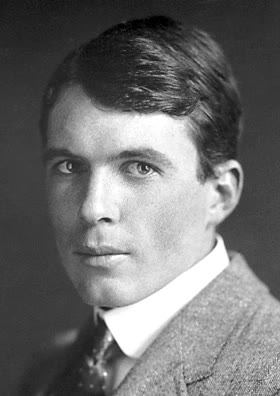
\includegraphics[width=\linewidth]{images/book4/bragg-wl.jpg}\par
{\footnotesize و. ل. براغ.}
\end{minipage}
\end{history}

\section{تمارين}

\begin{exercise}[$\star$]\label{exo:b3:x-ray-diffraction:1}
% ledger: lat:NaCl
من أجل \ce{NaCl} ($a = \qty{564.06}{pm}$)، احسب $d_{111}$ و$d_{200}$ و$d_{220}$.
\end{exercise}

\begin{exercise}[$\star$]\label{exo:b3:x-ray-diffraction:2}
% ledger: lat:Cu, xray:CuKa1
النحاس مكعب ممركز الأوجه حيث $a = \qty{361.50}{pm}$. باستعمال \babelsublr{Cu K$\alpha_1$} ($\lambda = \qty{154.06}{pm}$)،
احسب $2\theta$ لانعكاسيه الأولين، بعد تسميتهما.
\end{exercise}

\begin{exercise}[$\star$]\label{exo:b3:x-ray-diffraction:3}
أي الانعكاسات 100 و110 و111 و200 و210 و211 و220 حاضرة في
شبكة مكعبة P وI وF؟
\end{exercise}

\begin{exercise}[$\star$]\label{exo:b3:x-ray-diffraction:4}
أعطِ الأساس المقلوب لشبكة مستطيلة ثنائية البعد ضلعاها
$a$ و$b$، وارسم العقد المقلوبة الأولى.
\end{exercise}

\begin{exercise}[$\star\star$]\label{exo:b3:x-ray-diffraction:5}
% ledger: lat:W
يعطي فلز خطوطًا عند $2\theta = 40.27$ و58.26 و73.20 و87.01 و\ang{100.66} بإشعاع \babelsublr{Cu
K$\alpha_1$}. اقرن النمط، وجد نوع الشبكة و$a$.
\end{exercise}

\begin{exercise}[$\star\star$]\label{exo:b3:x-ray-diffraction:6}
% ledger: lat:KCl
بلورة من \ce{KCl} ($a = \qty{629.29}{pm}$) كثافتها المقيسة
\qty{1.99}{g/cm^3} (معطيات التمرين). جد $Z$.
\end{exercise}

\begin{exercise}[$\star\star$]\label{exo:b3:x-ray-diffraction:7}
عرض الخط (200) لمسحوق نانوي من \ce{NaCl} ($2\theta = \ang{31.70}$) هو \ang{0.40}،
ولا يساهم الجهاز بشيء. قدّر قياس البليرات.
\end{exercise}

\begin{exercise}[$\star\star$]\label{exo:b3:x-ray-diffraction:8}
للمركب \ce{CsCl} أيون \ce{Cs+} عند $(0,0,0)$ وأيون \ce{Cl-} عند $(\frac12,\frac12,\frac12)$ في خلية P. مع $f
\approx$ عدد الإلكترونات، احسب $F_{100}$ و$F_{110}$ ونسبة
شدتيهما (\omterm{def:b3:x-ray-diffraction:structure-factor}{عامل البنية} وحده). لماذا لا يكون \ce{CsCl} ممركز الجسم؟
\end{exercise}

\begin{exercise}[$\star\star$]\label{exo:b3:x-ray-diffraction:9}
بيّن أن الشبكة الممركزة القاعدة C (عقدة إضافية عند $(\frac12,\frac12,0)$) تُغيّب
الانعكاسات ذات $h + k$ الفردي.
\end{exercise}

\begin{exercise}[$\star\star\star$]\label{exo:b3:x-ray-diffraction:10}
فسّر لماذا لم يناقض اكتشاف سبائك في الثمانينيات تُظهر أنماط حيودها بقعًا حادة
ذات تناظر عشاري القيدَ البلوري، وما الذي
غيّره في تعريف البلورة.
\end{exercise}

\begin{exercise}[$\star\star\star$]\label{exo:b3:x-ray-diffraction:11}
بيّن أن \omterm{def:b3:x-ray-diffraction:space-group}{مستوي الانزلاق} في \babelsublr{\textit{P}$2_1/c$} يُغيّب الانعكاسات $h0l$ ذات $l$
الفردي.
\end{exercise}

\begin{exercise}[$\star\star\star$]\label{exo:b3:x-ray-diffraction:12}
المتماكب المرآوي النقي لا يمكن أن يتبلور أبدًا في \omterm{def:b3:x-ray-diffraction:space-group}{زمرة فضائية} تحتوي
\omterm{def:b3:point-groups:inversion}{مركز انقلاب} أو \omterm{def:b3:point-groups:mirror}{مستوي مرآة} أو \omterm{def:b3:x-ray-diffraction:space-group}{مستوي انزلاق}. لماذا؟ وفي أي نوع من الزمر الفضائية
يكون محصورًا، وماذا يقتضي قانون فريدل لتعيين ترتيبه الفراغي
المطلق؟
\end{exercise}

% keep the heading with its problem box, which fills a page by itself
\clearpage
\enlargethispage{3\baselineskip}
\section{مسألة: أيّ مسحوق أبيض؟}

\begin{problem}[{مسألة نهاية الأسبوع --- نمط مسحوق لملح مكعب مجهول:
المسافات، والقرننة، ووسيط الشبكة وهوية الملح، 
وقياس بليراته}]
\label{pb:b3:x-ray-diffraction:1}
% ledger: xray:CuKa1, lat:NaCl, lat:KCl, lat:KBr
مسحوق بلوري أبيض مجهول، يُعرف أنه \ce{NaCl} أو \ce{KCl} أو \ce{KBr}،
يعطي بإشعاع \babelsublr{Cu K$\alpha_1$} ($\lambda = \qty{154.059}{pm}$) الخطوط الآتية (معطيات
المسألة، محسوبة لهذا التمرين):
\begin{center}\small
\begin{tabular}{lcccccc}
\hline
\babelsublr{$2\theta$} بالدرجات & 28.342 & 40.512 & 50.178 & 58.632 & 66.380 & 73.692 \\
الشدة النسبية & 100 & 92 & 38 & 20 & 61 & 49 \\ \hline
\end{tabular}
\end{center}
لا يظهر أي خط آخر بين 20 و\ang{75}. وسائط الشبكة المرجعية:
\ce{NaCl} \qty{564.06}{pm}، \ce{KCl} \qty{629.29}{pm}، \ce{KBr} \qty{658.47}{pm}. الكتل المولية:
K 39.1، Na 23.0، Cl 35.5، Br \qty{79.9}{g/mol}.

\medskip\noindent\textbf{الجزء الأول --- المسافات.}
\begin{enumerate}
  \item احسب $\theta$ و$d$ للخط الأول.
  \item احسب $d$ لكل الخطوط.
  \item احسب النسب $\sin^2\theta/\sin^2\theta_1$.
  \item أي متتالية من الأعداد الصحيحة تجد؟
  \item هل يمكن أن يكون النمط لشبكة مكعبة أولية؟ وبأي $a$؟
  \item من أجل شبكة مكعبة أولية، أي عدد صحيح $N$ لا يمكن أن يظهر أبدًا؟ وهل
        يميّز النمط حتى الآن بين التفسيرين؟
\end{enumerate}

\medskip\noindent\textbf{الجزء الثاني --- الشبكة الحقيقية.}
\begin{enumerate}[resume]
  \item المرشحون الثلاثة كلهم شبكات F. اقرن الخطوط بمتتالية F.
  \item استنتج $a$ من الخط الأول.
  \item أي مرشح يوافق؟
  \item من أجل ذلك الملح، لماذا تغيب الانعكاسات الفردية كلها (111) و(311)؟
  \item هل يُظهر \ce{NaCl} الانعكاس (111)؟ وهل يُظهره \ce{KBr}؟
  \item فسّر لماذا يكون التفسير الأولي في الجزء الأول فخًا.
\end{enumerate}

\medskip\noindent\textbf{الجزء الثالث --- الكثافة والمحتوى.}
\begin{enumerate}[resume]
  \item كم وحدة صيغة تحتوي الخلية؟
  \item احسب الكثافة من الخلية.
  \item أعطِ عدد التناسق لكل أيون.
  \item احسب أقصر مسافة K--Cl.
  \item أي انعكاس سيظهر أولًا فوق \ang{75}؟
  \item لماذا تكون الشدات أقل فائدة من المواضع في تعرّف طور ما؟
\end{enumerate}

\medskip\noindent\textbf{الجزء الرابع --- التحسين وقياس البليرات.}
\begin{enumerate}[resume]
  \item لماذا يُفضَّل حساب وسيط الشبكة من خط ذي زاوية كبيرة؟
  \item احسب $a$ من الخط (420).
  \item عرض الخط (420) هو \ang{0.25} في $2\theta$ (العرض الآلي
        مهمل). قدّر قياس البليرات.
  \item هل يعرّض قياس بليرات قدره \qty{1}{\micro m} الخط تعريضًا قابلًا للقياس؟
  \item اذكر النتيجة: وسيط الشبكة المحسَّن من الخط (420)، 
        وهوية المسحوق.
\end{enumerate}
\end{problem}
